\documentclass[11pt]{article}
% fix quotes: https://tex.stackexchange.com/a/52353
\usepackage[english]{babel}
\usepackage{hyperref} % URLS
\usepackage{graphicx} % images
\usepackage{mathtools}
\usepackage{listings}
\usepackage{xcolor}
\usepackage{minted}
\usepackage{float}
 % no indent
\usepackage{parskip}
\usepackage[autostyle]{csquotes}
\usepackage{helvet}
% so we can stop latex hyphenating over new lines
%\usepackage[none]{hyphenat}
%\renewcommand{\familydefault}{\sfdefault}

% https://www.overleaf.com/learn/latex/Page_size_and_margins
\usepackage{geometry}
\geometry{
	a4paper,
	total={170mm,257mm},
	left=20mm,
	top=20mm,
}

% package instantiation
\MakeOuterQuote{"}
\hypersetup{
	colorlinks=true,
	linkcolor=blue,
	filecolor=magenta,
	urlcolor=cyan,
	citecolor=cyan,
}

% bibliography
% https://tex.stackexchange.com/questions/51434/biblatex-citation-order
% https://www.reddit.com/r/LaTeX/comments/k8tz0q/citation_in_wrong_numerical_order/
\usepackage[
    backend=biber,
    natbib=true,
    style=numeric,
    sorting=none
]{biblatex}
% \addbibresource{graphics.bib}

% opening
\title{\textbf{A 3D music visualisation in OpenGL using the Discrete Fourier Transform}}
\author{Matt Young \\ s4697249 \\ m.young2@uqconnect.edu.au}
\date{March 2024}

\begin{document}
\maketitle

\begin{abstract}
    Constructing computer graphics from music has important implications in the field of live entertainment.
    The Discrete Fourier Transform (DFT), often computed via the Fast Fourier Transform (FFT), is the typical
    method to convert time domain audio signals to a frequency domain spectrum. With this spectral data comes
    an almost unlimited number of ways to interpret it and construct a visualisation. In this paper, I
    investigate applying the DFT to construct a semi real-time audio visualisation using OpenGL. The
    visualisation consists of offline spectral data that is rendered in real-time in the form of "bars" with
    emissive lighting, and a set of pre-programmed camera moves computed via spherical linear interpolation.
\end{abstract}

\tableofcontents

\section{Introduction}
Since the first music video in (YEAR) (CITE), there has been broad interest in constructing "music
visualisers": the process of building an often real-time visual representation of the audio.

- creative and technical
- music visualisers used by live musicians
- many different ways to interpret audio signals
- demoscene inspiration

\subsection{Visual inspiration}
The particular music visualiser I aim to construct is an improved version of the "spectrum of bars" once used
by Canadian record label Monstercat, shown in Figure \ref{monstercat}. The label has since transitioned away
from this computational music visualiser, and instead use custom music videos.

\begin{figure}[H]
\centering
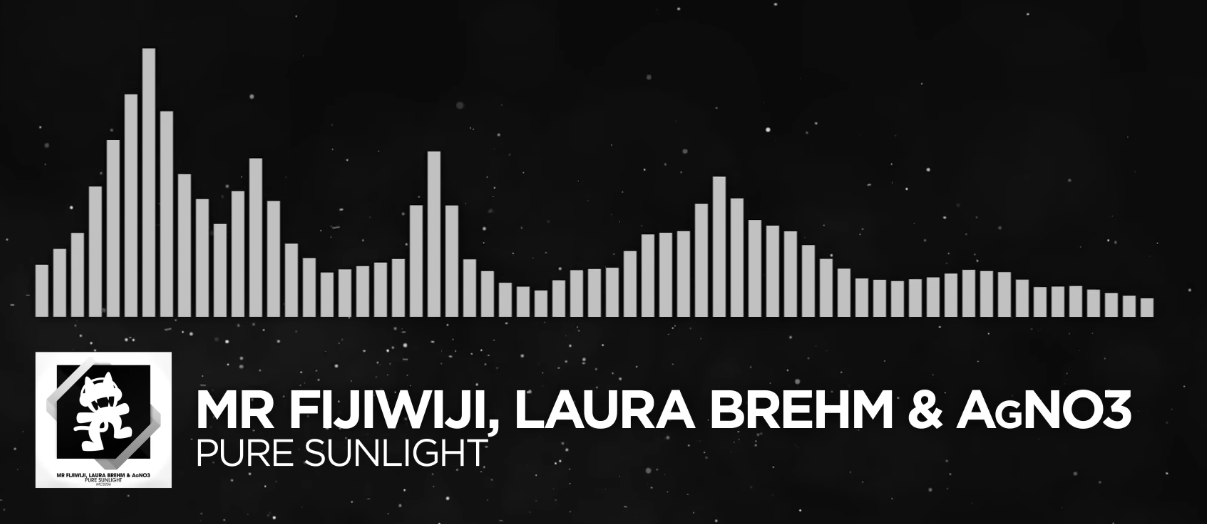
\includegraphics[width=384px]{img/monstercat.png}
\caption{Visualisation of the song "Pure Sunlight", CITATION.}
\label{monstercat}
\end{figure}

- demoscene inspiration

\section{Architecture overview}
\subsection{Overall description of sub-applications}
The visualiser itself is developed and tested in a Linux environment, and is split into two sub-applications:
the visualiser itself (written in C++20), and the analysis script (written in Python). Signal processing is a
very complex subject, and real-time ("online") signal processing is even more so. Python generally has simpler
tools to address signal processing problems, such as NumPy and SciPy, so the signal processing part was moved
offline into a Python script.

(DIAGRAM)

The analysis script is first run that reads a FLAC (CITATION) audio file, and produces a Cap'n Proto (CITATION)
encoded binary file containing the necessary data to render a spectrum for the chosen song. Each song consists
of a directory containing one audio file, \verb|audio.flac|, and one spectral data file, \verb|spectrum.bin|.
These are stored in the \verb|data| directory. For example: \\
\verb|data/songs/LauraBrehm_PureSunlight/{audio.flac},{spectrum.bin}|

(DIRECTORY TREE)

Free Lossless Audio Codec (FLAC) is a lossless audio compression and container format. It was chosen because
(REASONS).

Cap'n Proto is a binary serialisation format that is regarded as a faster successor to Protocol Buffers.
Compared to Protocol Buffers, which are also a widely used binary serialisation format, Cap'n Proto has the
added benefit of requiring zero decode time and supporting very fast in-memory access. This is perfect for the
spectral data, which needs to be written once by the Python code, and re-read continuously by the C++
rendering code. Some of this reading takes place in the audio callback, which could be regarded as a soft
real-time function, and hence requiring very minimal overhead.
\footnote{Additionally, Cap'n P integrates nicely with my editor, Neovim, which was one of the bigger reasons
for its selection.}

The FLAC file for a typical song weighs in at around 10 MB, and the spectral data is only around 200 KiB
thanks to Cap'n Proto's packed stream writing feature. \footnote{Due to its speed, Cap'n P has to make some
trade-offs in regards to message size vs. speed, usually preferring larger messages. Since my files are
checked into Git, I used packed message writing to prefer smaller messages with an ever so slightly longer
decode time.}

\subsection{Visualiser}
The visualiser is what we see on the screen, the real-time rendering system that displays the bars, once the
spectral data has been computed. It is written in C++20 using OpenGL, and is built using industry standard
tools CMake, Ninja and the Clang compiler. It uses a number of open-source libraries:
\begin{itemize}
	\item SDL2: Platform window management, keyboard/mouse inputs, OpenGL context creation
	\item glad: For OpenGL function loading and feature queries
    \item glm: The OpenGL maths library, used for computing transforms and its matrix/vector types
    \item Cap'n Proto: An extremely fast data serialisation format, used to transport data between Python and
        C++.
\end{itemize}

\subsection{Analysis script}
The analysis script is written in Python, and computes the spectral data itself. It takes a FLAC file, and
computes the spectral data necessary to render the bars. It also uses a number of open source libraries:
\begin{itemize}
    \item NumPy
    \item SciPy
    \item spectrum.py
    \item Cap'n Proto
\end{itemize}

\section{Signal processing}
The overarching goal of the signal processing is to turn a time-domain audio signal into a frequency domain
spectrogram, similar to the Monstercat visualiser shown in Figure \ref{monstercat}. This turns out to actually
be quite an involved process, so this section will essentially a whirlwind tour of audio signal processing!

\subsection{Fourier transforms and the DFT}

\subsection{Decoding and chunking audio}
In order for the Fourier transform to be possible, a \textit{chunk} of audio needs to be processed. In other
words, we can't just process individual samples since we're doing a time-domain to frequency-domain
transform. After decoding the FLAC audio using the \verb|audiofile| library, the audio samples are then split
into chunks/blocks of 1024 samples using NumPy. Additionally, the stereo signal is transformed into a mono
signal by averaging the left/right channels, since multi-channel FFTs are much more complicated.

This is all just a few lines of Python:
\begin{minted}{python}
    # load audio
    signal, sampling_rate = audiofile.read(song_path, always_2d=True)
    # assume a stereo signal, let's mix it down to mono
    mono = np.mean(signal, axis=0)
    # split signal into chunks of BLOCK_SIZE
    blocks = np.split(mono, range(BLOCK_SIZE, len(mono), BLOCK_SIZE))
\end{minted}


\subsection{Power spectrum and periodogram}

\subsection{Conversion to dBFS}

\subsection{Sampling and binning spectral data}

\section{Computer graphics}

\section{Results}

\section{Conclusion}

\section{References}
\printbibliography[heading=none]

\end{document}
